\begingroup
\makeatletter\tagsleft@true\let\veqno\@@leqno\makeatother
\clearpage\SourceLeaf{318}\NoSourceHead
\SourceGroup{III}
\HistoricTitle{[IN DEN KLEINSTEN THEILEN ÄHNLICHE ABBILDUNG DER FLÄCHE\\ EINER ELLIPSE AUF DIE FLÄCHE EINES KREISES.]}
\HistoricCitation{[Aus Handbuch 19, Be, Kleine Aufsätze aus verschiedenen Theilen\\ der Mathematik, Angefangen im May 1809.]}
\noindent {\small[S 172]}
\begin{center}\bfseries Anziehung in der Ebne, umgekehrt dem Abstande proport[ional].\end{center}
\par\indent Es sei eine in sich selbst zurückkehrende Linie $=L$ aufgegeben. Man wünscht allgemein, jede andere $L'$ zu bestimmen, so dass der Flächenring zwischen beiden gar keine Anziehung auf den innern Raum bewirke.
\par\indent\textsubscript{*} Die allgemeine Auflösung kommt darauf an, dass, die Coordinaten jedes Punctes in $L$ durch $x,y$ ferner $x+yi$ durch $t$ und eine unbestimmte Grösse durch $\varphi$ und $\cos\varphi+i\sin\varphi$ durch $\varepsilon$ bezeichnet, $t$ in der Gestalt einer Function von $\varepsilon$ dargestellt werde, $t=f\varepsilon$. Es ist dann allgemein, $t'$ die $x'+iy'$ in $L'$ bezeichnend, $t'=af\varepsilon$.\textsuperscript{*}
\par\medskip\noindent
\begin{minipage}[c]{.25\linewidth}\centering
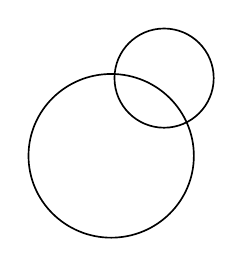
\begin{tikzpicture}[x=1.05cm,y=1.05cm,line width=.6pt]
\draw (0,0) ellipse[x radius=1,y radius=.99];
\draw (.64,.94) circle[radius=.60];
\end{tikzpicture}
\end{minipage}\hfill
\begin{minipage}[c]{.70\linewidth}
\setlength{\parindent}{1.2em}
\par\indent\textsubscript{**} Schönes Theorem. Wenn eine in sich zurückk[ehrende] Linie $L$ in jedem Puncte des unendlichen Raumes dieselbe Anziehung ausübt, wie eine andere Linie $L'$, und beide einander schneiden, so gilt jene Gleichheit auch innerhalb des gemeinschaftlichen Raumes.
\end{minipage}
\par\medskip\noindent
\begin{minipage}[c]{.70\linewidth}
\setlength{\parindent}{1.2em}
\par\indent Vielleicht etwas ähnliches auch wenn sie sich nicht schneiden sondern nur einschliessen?\textsuperscript{**}[*)]
\end{minipage}\hfill
\begin{minipage}[c]{.25\linewidth}\centering
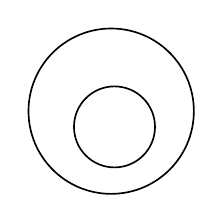
\begin{tikzpicture}[x=1.05cm,y=1.05cm,line width=.6pt]
\draw (0,0) circle[radius=1];
\draw (.04,-.19) circle[radius=.49];
\end{tikzpicture}
\end{minipage}
\par\bigskip\noindent\rule{.25\linewidth}{.4pt}\par\smallskip
{\small\par\indent [*) In der Handschrift ist der oben zwischen \textsubscript{*}\ \textsuperscript{*} gesetzte Absatz mit Bleistift, der zwischen \textsubscript{**}\ \textsuperscript{**} gesetzte mit Tinte durchstrichen.]\par}
\clearpage\SourceLeaf{319}\ArithmeticHead{312}{L}{ANALYSIS.\quad NACHLASS.}
\NumberedItem{2}
\noindent {\small[S. 173]}
\par\indent Die Puncte einer Ellipse werden durch
\[2t=(a+b)\varepsilon+(a-b)\varepsilon^{-1}\]
\noindent dargestellt.
\par\indent Hier wird $t$ durch die Gleichung bestimmt
\[\begin{gathered}
(t+\surd(tt-(aa-bb)))^n\pm(t-\surd(tt-(aa-bb)))^n\\
=(a+b)^n\pm(a-b)^n.
\end{gathered}\]
\NumberedItem{3}
\noindent {\small[S. 176]}
\par\indent Es sein $x,y$ indef[inite] die Coordinaten der Puncte einer Ellipse, deren Halbaxen $=a,b$ und $x+yi=T$, ferner
\[\frac{aa-bb}{2(aa+bb)}=k.\]
\noindent Es sei ferner $t$ Function eines unbestimmten Winkels $=\cos\varphi+i\sin\varphi$. Man soll $T$ in die Form
\begin{equation}
t+At^3+Bt^5+Ct^7\,{.}{.}{.}\tag*{[1]}
\end{equation}
\noindent bringen.
\par\indent Setzt man $x-yi=T'$, so wird
\begin{equation}
T'=t^{-1}+At^{-3}+Bt^{-5}+Ct^{-7}\,{.}{.}{.}\tag*{[2]}
\end{equation}
\noindent und die Coefficienten werden bestimmt durch die Gl[eichung]
\begin{equation}
k(TT+T'T')=TT'-\frac{2aabb}{aa+bb}\mathpunct{\raisebox{.5ex}{.}}\tag*{[3]}
\end{equation}
\noindent Es findet sich
\clearpage\SourceLeaf{320}\ArithmeticHead{313}{R}{{\scriptsize ABBILDUNG DER ELLIPSE AUF DEN KREIS.}}
\[\begin{aligned}
T={}&t\\
&+t^3(k-2k^3+3k^5-k^7\\
&+t^5(2kk-9k^4+24k^6-35k^8\\
&+t^7(5k^3-36k^5+142k^7-348k^9\\
&+t^9(14k^4-140k^6+740k^8\\
&+t^{11}(42k^5-540k^7+3600k^9\\
&+t^{13}(132k^6-2079k^8+16786k^{10}.\\
&+t^{15}(429k^7-8008k^9
\end{aligned}\]
\[\begin{aligned}
t={}&T-T^3(k-2k^3+3k^5-k^7\\
&+T^5(k^2-3k^4+6k^6-7k^8\\
&-T^7(k^3-4k^5+10k^7-24k^9
\end{aligned}\]
\[\begin{aligned}
TT={}&tt\\
&+t^4(2k-4k^3+6k^5-2k^7\\
&+t^6(5kk-22k^4+58k^6-84k^8\\
&+t^8(14k^3-98k^5+380k^7-920k^9\\
&+t^{10}(42k^4-408k^6+2115k^8\\
&+t^{12}(132k^5-1650k^7+10780k^9\\
&+t^{14}(429k^6-6578k^8\\
&+t^{16}(1430k^7-26026k^9\\
&+t^{18}(4862k^8\\
&+t^{20}(16796k^9
\end{aligned}\]
\noindent {\small[S. 177]}
\par\indent Die erste senkrechte Reihe in $T$ ist
\[=\frac{1-(1-4ktt)^{\frac12}}{2kt},\]
\noindent die zweite
\[=\frac{1-(1-2ktt-2kkt^4)(1-4ktt)^{-\frac12}}{2t^3},\]
\noindent die dritte
\[=\frac{k}{t^5}\left\{1-ktt-(1-7ktt+12kkt^4-2k^3t^6-k^4t^8).\,(1-4ktt)^{-\frac32}\right\}.\]
\noindent Es wird hier der constante Theil von $TT'$
\par\medskip\noindent X1.\hfill40
\clearpage\SourceLeaf{321}\ArithmeticHead{314}{L}{ANALYSIS.\quad NACHLASS.}
\[\begin{aligned}
&=1+kk\quad\ast\quad-k^6-k^8+k^{10}\,{.}{.}{.}\\
&=1:(1-kk+k^4\quad\ast\quad\ast\quad-k^{10}\,{.}{.}{.}
\end{aligned}\]
\clearpage
\endgroup
